%==================================================================================================
\chapter{Análise numérica para dinâmica não linear dos sólidos} \label{EGDS}
%==================================================================================================

Inicialmente considere um corpo deformável, idealizado como um meio contínuo que, em sua configuração inicial é denotado por $\Omega_0$ e em sua configuração atual é denotado por $\Omega$, conforme ilustrado na Figura \ref{fig:Cont}. Para se mapear os pontos que compõem o corpo em relação a uma origem preestabelecida utiliza-se $\BB{x}$ e $\BB{y}$ para denotar as coordenadas de $\Omega_0$ e $\Omega$, respectivamente. Já para se mapear $\BB{y}$ em função de $\BB{x}$ existe uma função $\BB{f}$ tal que $\BB{y}=\BB{f}(\BB{x})$, denominada como função de mudança de configuração.

\begin{figure}[h!]
    \centering
    \caption{Configurações inicial e atual de um corpo deformável.}
    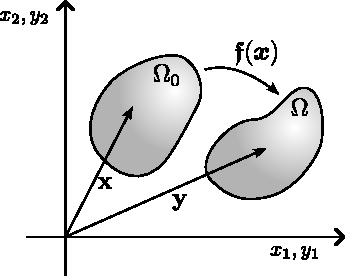
\includegraphics[width=.4\linewidth]{Figuras/Cont.pdf}
    \\Fonte: Autoria Própria (\the\year).
    \label{fig:Cont}
\end{figure}

Para um ponto $\BB{x}$ na vizinhança de $\BB{x}_0$, pode-se dizer que:

\begin{equation}
    \BB{y}(\BB{x})=\fmc(\BB{x}_0)+\Nx\fmc|_{\BB{x}_0}\cdot d\BB{x}\text{,}
\end{equation}

\noindent em que $\FMC=\Nx\fmc$ é o gradiente de mudança de configuração. Assim, pode-se obter uma expressão que transforme um vetor $d\BB{x}$ na configuração inicial em um vetor $d\BB{y}$ na atual:

\begin{equation}
    d\BB{y}=\FMC\cdot d\BB{x}\text{,}\label{eq:dyAdx}
\end{equation}

\noindent o que permite escrever o quadrado da norma de $d\BB{y}$ como:

\[
    \norm{d\BB{y}}^2=dy^2=d\BB{y}\trans\cdot d\BB{y}=(\FMC\cdot d\BB{x})\trans\cdot(\FMC\cdot d\BB{x})=d\BB{x}\trans\cdot\FMC\trans\cdot\FMC\cdot d\BB{x}
\]

Subtraindo-se $dx^2=\norm{d\BB{x}}^2$ de ambos os lados da igualdade obtém-se:

\begin{equation}
    dy^2-dx^2=d\BB{x}\trans\cdot(\FMC\trans\cdot\FMC-\BB{I})\cdot d\BB{x}\text{,}
    \label{eq:difdxdy}
\end{equation}

\noindent em que $\BB{I}$ é o tensor identidade de segunda ordem e $\BB{C}=\FMC\trans\cdot\FMC$ é o tensor de alongamento à direita de Cauchy-Green. Dessa maneira, pode-se substituir $\BB{C}$ em \eqref{eq:difdxdy} e dividir por $2dx^2$, obtendo-se:

\[
    \frac{1}{2}\frac{dy^2-dx^2}{dx^2}=\frac{1}{2}\frac{d\BB{x}\trans\cdot(\BB{C}-\BB{I})\cdot d\BB{x}}{dx^2}\text{.}
\]

\noindent Tomando um versor na direção de $d\BB{x}$ ($\BB{u}=d\BB{x}/\norm{d\BB{x}}$), tem-se que:

\begin{equation}
    \frac{1}{2}\frac{dy^2-dx^2}{dx^2}=\BB{u}\trans\cdot\left(\frac{1}{2}(\BB{C}-\BB{I})\right)\cdot\BB{u}\text{.}
\end{equation}

Assim, define-se o tensor de deformações de Green-Lagrange como:

\begin{equation}
    \mathbb{E}=\frac{1}{2}(\BB{C}-\BB{I})\text{,}
    \label{eq:CSD-DefGreenLagr}
\end{equation}

\noindent que se trata de uma medida de deformação objetiva, ou seja, não registra deformações em situação de movimento de corpo rígido.

Outra medida de deformação interessante é a medida de deformação volumétrica ($\varepsilon_V$). Para isso considere o elemento infinitesimal em suas configurações inicial e atual ilustrado na Figura \ref{fig:MudVol}.

\begin{figure}[h!]
    \centering
    \caption{Mudança de volume de um elemento infinitesimal.}
    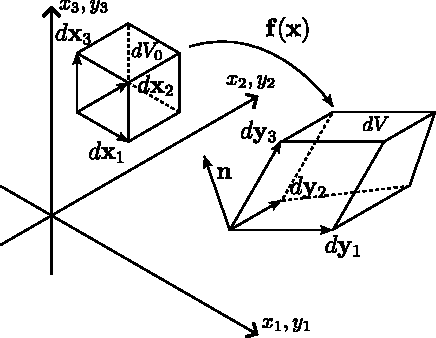
\includegraphics[width=0.5\linewidth]{Figuras/MudVol.pdf}
    \\Fonte: Autoria Própria (\the\year).
    \label{fig:MudVol}
\end{figure}

Logo o valor de $\varepsilon_V$ pode ser obtido através da relação entre o volume inicial e atual desse elemento como:

\begin{equation}
    \varepsilon_V=\frac{dV-dV_0}{dV_0}\text{.}
\end{equation}

O volume do elemento em ambas as configurações pode ser obtido por meio do produto misto dos vetores que formam o mesmo, ou seja:

\begin{subequations}
    \begin{equation}
        dV_0=d\BB{x}_1\cdot(d \BB{x}_2\times d\BB{x}_3)\text{,}
    \end{equation}
    \begin{equation}
        dV=d\BB{y}_1\cdot(d \BB{y}_2\times d\BB{y}_3)\text{,}
    \end{equation}
\end{subequations}

Conhecendo a transformação expressa em \eqref{eq:dyAdx} e fazendo as devidas simplificações pode-se obter que:

\begin{equation}
    dV=\det{(\FMC)}dV_0=JdV_0\text{,}\label{eq:RelVol}
\end{equation}

\noindent em que $J=\det{(\FMC)}$ é o Jacobiano da mudança de configuração.

Na sequência procura-se obter uma expressão que indique a mudança de área nas diferentes configurações. Assim, considere um cilindro infinitesimal ilustrado na figura \ref{fig:Nanson}.

\begin{figure}[h!]
    \centering
    \caption{Mudança de configuração em um cilindro infinitesimal.}
    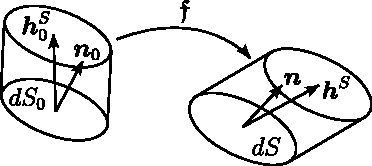
\includegraphics[width=.45\linewidth]{Figuras/Nanson.pdf}
    \\Fonte: Autoria Própria (\the\year).
    \label{fig:Nanson}
\end{figure}

Nesse contexto, a área vetorial pode ser entendida como seu valor absoluto na direção de sua normal ($d\BB{S}_0=dS_0\BB{n}_0$ e $d\BB{S}=dS\BB{n}$). Logo o volume do cilindro é dado pelo produto escalar da área vetorial com o vetor que define a altura do cilindro ($dV_0=d\BB{S}_0\cdot\BB{h}^S_0$ e $dV=\BB{S}\cdot\BB{h}^S$). Conhecendo as relações \eqref{eq:dyAdx} e \eqref{eq:RelVol}, pode-se obter que:

\begin{equation}
    \BB{n}dS=J\FMC\Ttrans\cdot\BB{n}_0dS_0\text{,}\label{eq:Nanson}
\end{equation}

\noindent que é conhecida como a Equação de Nanson.

Com esse embasamento é possível apresentar os conceitos de energia nas descrições Euleriana e Lagrangiana Total. Assim, para se obter a equação do equilíbrio local de um elemento na descrição Euleriana, considere um elemento infinitesimal sujeito à ação de uma força de corpo (ou de volume) $\BB{c}$, conforme ilustrado no diagrama de corpo livre da Figura \ref{fig:CorpoLivreSolido}, que apresenta somente as forças atuantes na direção $y_1$.

\begin{figure}[h!]
    \centering
    \caption{Forças atuantes em um elemento infinitesimal na direção $y_1$.}
    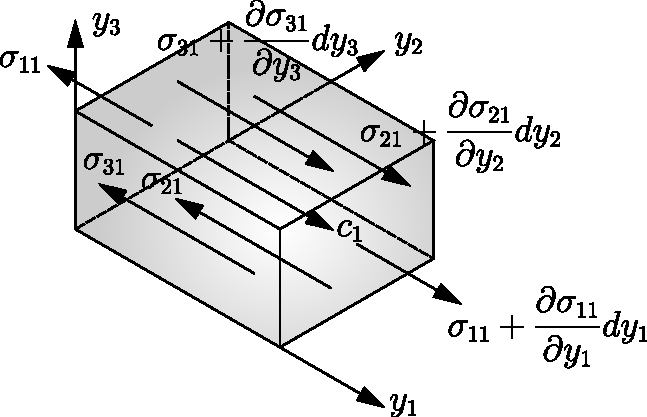
\includegraphics[width=.5\linewidth]{Figuras/CorpoLivreSolido.pdf}
    \\Fonte: Autoria Própria (\the\year).
    \label{fig:CorpoLivreSolido}
\end{figure}

Fazendo o equilíbrio das forças nessa direção e realizando as devidas simplificações tem-se:

\[\der{\sigma_{11}}{y_1}+\der{\sigma_{21}}{y_2}+\der{\sigma_{31}}{y_3}+c_1=\rho\ddot{y}_1\text{,}\]

\noindent que, expandindo analogamente para as demais direções tem-se:

\begin{equation}
    \Ny\cdot\tens\trans+\BB{c}=\rho\ddot{\BB{y}}\text{,}
    \label{eq:EqLocEu}
\end{equation}

\noindent a qual representa a equação do equilíbrio local na descrição Euleriana.

Integrando a equação \eqref{eq:EqLocEu} em $\Omega$ e aplicando o teorema da divergência obtém-se:

\begin{equation}
    \int_\Gamma{\tens\trans\cdot\BB{n}d\Gamma}+\int_\Omega{\BB{c}d\Omega}=\int_\Omega{\rho\ddot{\BB{y}}d\Omega}
    \text{,}
    \label{eq:EqGlobEu}
\end{equation}

\noindent onde $\Gamma=\partial\Omega$ é a fronteira do domínio de análise. Essa equação representa o equilíbrio global na descrição Euleriana.

Já em uma descrição Lagrangiana Total, será necessário transformar os termos dependentes da configuração atual para outros dependentes da configuração inicial. Assim, pode-se reescrever a Equação \eqref{eq:EqGlobEu} levando em consideração as Equações \eqref{eq:RelVol} e \eqref{eq:Nanson}:

\begin{equation}
    \int_{\Gamma_0}{J\tens\trans\cdot\FMC\Ttrans\cdot\BB{n}_0d\Gamma_0}+\int_{\Omega_0}{J\BB{c}d\Omega_0}=\int_{\Omega_0}{J\rho\ddot{\BB{y}}d\Omega_0}
    \text{.}
\end{equation}

\noindent Sendo $\BB{c}^0=J\BB{c}$ as forças de corpo na configuração inicial, $\rho_0=J\rho$ a densidade inicial e $\BB{P}=J\FMC^{-1}\cdot\tens$ o primeiro tensor de tensões de Piola-Kirchhoff, tem-se que:

\begin{equation}
    \int_{\Gamma_0}{\BB{P}\trans\cdot\BB{n}_0d\Gamma_0}+\int_{\Omega_0}{\BB{c}^0d\Omega_0}=\int_{\Omega_0}{\rho_0\ddot{\BB{y}}d\Omega_0}\text{,}
\end{equation}

\noindent que representa a equação do equilíbrio global na descrição Lagrangiana Total.

Retornando a integral sob a fronteira $\Gamma_0$ para $\Omega_0$ por meio do Teorema da Divergência e tomando um elemento infinitesimal de volume, pode-se obter a equação do equilíbrio local na descrição Lagrangiana Total:

\begin{equation}
    \Nx\cdot\BB{P}\trans+\BB{c}^0=\rho_0\ddot{\BB{y}}\text{, ou}
\end{equation}

%==================================================================================================
\section{Abordagem energética para determinação do ponto de equilíbrio}
%==================================================================================================

Em se tratando de sólidos de comportamento hiperelástico, dada a natureza das leis constitutiva e à adequação da descrição Lagrangiana, é conveniente o uso de abordagens energéticas de modo a obter o equacionamento em forma fraca, seguido da aplicação da técnica de elementos finitos e de processos para solução numérica do sistema resultante. Para tal, deve-se primeiramente definir o conceito de energia total ($\Pi$) de um sistema, que pode ser entendido como a soma de todas as parcelas de energia relevantes ao problema. Nos casos mais comuns, tem-se uma parcela de energia potencial das forças externas atuantes no corpo ($\mathbb{P}$), uma parcela de energia de deformação elástica ($\mathbb{U}$) e parcela de energia cinética ($\mathbb{K}$). Dessa forma, o funcional de energia total é dado por:

\begin{equation}
    \Pi=\mathbb{P}+\mathbb{U}+\mathbb{K}\text{.}
    \label{FuncionalEnergia}
\end{equation}

Busca-se encontrar a configuração de equilíbrio do sólido, e para tal, a conservação da energia deve ser respeitada. Dessa forma postula-se o primeiro teorema variacional, que aponta que, para se obter o equilíbrio em um sólido sujeito a forças externas conservativas, a primeira variação da energia total deve ser nula para qualquer variação admissível nas incógnitas do problema ($\DOF$), ou seja:

\begin{equation}
    \delta^{(1)}\Pi=0\forall\delta\DOF|\delta\DOF=\BB{0}\text{ em }\Gamma_D\text{,}
\end{equation}

\noindent em que $\Gamma_D$ é a parcela da fronteira onde os deslocamentos são prescritos. Já o segundo teorema trata-se da estabilidade desse equilíbrio, onde para se atingir o equilíbrio estável a segunda variação da energia total deve ser positiva para qualquer variação admissível, ou seja:

\begin{equation}
    \delta^{(2)}\Pi>0\forall\delta\DOF|\delta\DOF=\BB{0}\text{ em }\Gamma_D\text{.}
\end{equation}

Sendo assim, primeiramente procura-se anular a primeira variação da energia total:

\begin{equation}
    \delta\Pi=\delta\mathbb{P}+\delta\mathbb{U}+\delta\mathbb{K}=0\text{,}
\end{equation}

\noindent o que leva à necessidade de se determinar a primeira variação de $\mathbb{U}$. Para isso, é necessária a consideração de um modelo constitutivo que permita, juntamente com as demais equações da cinemática do modelo estrutural, descrever a evolução da energia de deformação em função das variáveis principais do problema. Um possível modelo constitutivo é o de Saint-Venant-Kirchhoff, dado por:

\begin{equation}
    u_e^{SVK}=\frac{\Stens:\mathbb{E}}{2}\text{,}
\end{equation}

\noindent no qual $\Stens$ é o tensor de Piola-Kirchhoff de segunda espécie, calculado como:

\begin{equation}
    \Stens=\tensCon:\mathbb{E}\text{,}
    \label{eq:CSD-S}
\end{equation}

\noindent sendo $\tensCon$ o tensor constitutivo de quarta ordem:

\begin{equation}
    \tensCon=2G\mathbb{I}+\frac{2G\nu}{1-2\nu}\BB{I}\otimes\BB{I}
\end{equation}

\noindent em que $\nu$ é o coeficiente de Poisson e $G$ é o módulo de elasticidade transversal, dado em função do módulo de elasticidade longitudinal (ou Módulo de Young) $E$ como:

\begin{equation}
    G=\frac{E}{2(1+\nu)}\text{.}
\end{equation}

Assim, as parcelas de energia ficam dadas por:

\begin{subequations}
    \begin{align}
         & \mathbb{U}=\frac{1}{2}\intDomi{\Stens:\mathbb{E}}\text{,}                  \\
         & \mathbb{P}=-\BB{F}^a\cdot\BB{Y}^a-\intFronti{\BB{t}\cdot\BB{y}^m}\text{ e} \\
         & \mathbb{K}=\frac{1}{2}\intDomi{\rho_0\norm{\dBB{y}}^2}\text{,}
    \end{align}
\end{subequations}

\noindent onde $\Omega_0$ é o domínio de análise em sua configuração inicial, cuja fronteira é $\Gamma_0=\partial\Omega_0$, $\BB{F}^a$ é uma força concentrada aplicada sobre um ponto $a$, cuja posição atual é $\BB{Y}^a$, $\BB{t}$ é uma força distribuída sobre uma superfície média da casca ($\BB{y}$) e $\rho_0$ é a massa específica inicial do contínuo.

%\noindent O Apêndice \ref{Ap:CSD} trata de forma mais detalhada o comportamento para casos multiaxiais.

%==================================================================================================
\section{Método dos Elementos Finitos Posicional Aplicado a Elementos de Casca} \label{MEFP}
%==================================================================================================

Os elementos de casca podem ser entendidos como aqueles em que uma de suas dimensões é muito menor que as demais. Assim, é possível tomar como referência a superfície média do elemento para mapear os pontos que o compõem, facilitando a descrição.

A formulação que será apresentada a seguir segue a cinemática de Reissner-Mindlin, levando em consideração as deformações causadas pelas tensões de cisalhamento nas direções transversais ao elemento, e foi proposta por \citeonline{coda2007alternative}, já tendo sido aplicada com sucesso ao contexto da interação fluido-estrutura por \citeonline{sanches2011acoplamento,sanches2013unconstrained} e \citeonline{fernandes2019ale}.
%\textcolor{red}{Deixe a parcela dissipativa de fora...}

%==================================================================================================
\subsection{Cinemática de Reissner-Mindlin}
%==================================================================================================

As configurações inicial a atual de um elemento de casca podem ser descritas mapeando-se um elemento plano e de dimensões unitárias, definido em um espaço de coordenadas paramétricas adimensionais ($\BB{\xi}$), empregando-se para tal, as funções de forma polinomiais definidas no espaço de coordenadas $\BB{\xi}$, como ilustrado na Figura \ref{fig:Mapeamento}.

\begin{figure}[h!]
    \centering
    \caption{Mudança de configuração.}
    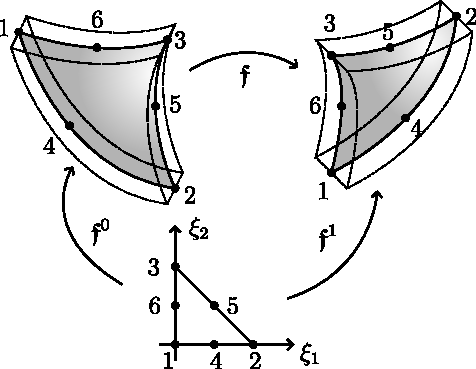
\includegraphics[width=.4\linewidth]{Figuras/Mapeamento.pdf}
    \\Fonte: Autoria Própria (\the\year).
    \label{fig:Mapeamento}
\end{figure}

Para isso, realiza-se primeiramente o mapeamento dos pontos da superfície média do elemento para a configuração inicial de coordenadas $\BB{x}^m$ e para a configuração atual, de coordenadas $\BB{y}^m$:

\begin{subequations}
    \begin{align}
         & \fmc^{m0}=\BB{x}^m=\BB{X}_aN_a(\xi_1,\xi_2)\text{,} \\
         & \fmc^{m1}=\BB{y}^m=\BB{Y}_aN_a(\xi_1,\xi_2)\text{,}
    \end{align}
\end{subequations}

\noindent onde $\fmc^{m0}$ e $\fmc^{m1}$ são as funções de mapeamento da superfície média para as configurações inicial a atual, respectivamente, $\BB{X}_a$ e $\BB{Y}_a$ são as coordenadas dos nós $a$, pertencentes à superfície média nas configurações inicial e atual, respectivamente, e $N_a(\xi_1,\xi_2)$ é a função de forma associada ao nó $a$.

Já os pontos fora da superfície média, são mapeados com auxílio de vetores generalizados $\BB{v}^0$ e $\BB{v}^1$, sendo as funções de mapeamento para qualquer ponto, para as configurações inicial e atual, dadas por:

\begin{subequations}
    \begin{align}
         & \fmc^0=\BB{x}^m(\xi_1,\xi_2)+\BB{v}^0(\xi_1,\xi_2,\xi_3)\text{ e} \\
         & \fmc^1=\BB{y}^m(\xi_1,\xi_2)+\BB{v}^1(\xi_1,\xi_2,\xi_3)\text{,}
    \end{align}
\end{subequations}

\noindent onde $\BB{v}^0$ é normal à superfície média inicial ao ponto mapeado, e enquanto $\BB{v}^1$ é o vetor, não necessariamente normal à superfície média, que liga o ponto da superfície média de coordenadas $(\xi_1,\xi_2)$ ao ponto mapeado na configuração atual. Empregando-se as mesmas funções de forma do elemento plano para representar esses vetores, escrevem-se as aproximações:

\begin{subequations}
    \begin{align}
         & \BB{v}^0=\frac{h_0}{2}\BB{w}^0\xi_3\text{ e}                \\
         & \BB{v}^1=\frac{h_0}{2}\BB{w}^1[\xi_3+\alpha\xi_3^2]\text{,}
    \end{align}
\end{subequations}

\noindent sendo $h_0$ a espessura inicial da casca, $\BB{w}^0$ e $\BB{w}^1$ os vetores generalizados adimensionais na configuração inicial e atual, respectivamente, e $\alpha$ é um enriquecimento nodal inserido ao problema com a finalidade de evitar travamento volumétrico, o qual representa a taxa de variação linear da deformação na direção da espessura. Essas variáveis podem ser aproximadas via funções de forma como:

\begin{subequations}
    \begin{align}
         & \BB{w}^0(\xi_1,\xi_2)=\BB{V}^0_aN_a(\xi_1,\xi_2)\text{,}  \\
         & \BB{w}^1(\xi_1,\xi_2)=\BB{V}^1_aN_a(\xi_1,\xi_2)\text{ e} \\
         & \alpha(\xi_1,\xi_2)=\Alpha_aN_a(\xi_1,\xi_2)\text{,}
    \end{align}
\end{subequations}

\noindent em que $\BB{V}^0_a$, $\BB{V}^1_a$ e $\Alpha_a$ são os valores nodais das variáveis associados ao nó $a$ \cite{sanches2013unconstrained,sanches2014fluid}. É importante notar que $\BB{w}^0$ é unitário e normal à superfície média, enquanto $\BB{w}^1$ não é mais necessariamente normal à superfície média nem unitário.

Sendo assim, o problema possui como graus de liberdade as posições nodais atuais da superfície média ($\BB{Y}_a$), os valores nodais do vetor generalizado adimensional na configuração atual ($\BB{V}^1_a$) e o valor nodal da taxa de variação linear de deformação na direção da espessura ($\Alpha_a$).

Além disso, torna-se necessário determinar o gradiente da função de mudança de configuração. Para isso note que $\fmc(\BB{x},t)=\fmc^1((\fmc^0)^{-1},t)$, portanto é possível se obter o gradiente da função de mudança de configuração como $\FMC=\FMC^1\cdot(\FMC^0)^{-1}$, em que $\FMC^0=\Nxi\fmc^0$ e $\FMC^1=\Nxi\fmc^1$.

Considerando-se o princípio da conservação da energia, tem-se:

\begin{equation}
    \delta\Pi=\der{\Pi_0}{\DOF}\cdot\delta\DOF=0\text{,}
\end{equation}

\noindent em que $\DOF$ representa o vetor que contém todos os graus de liberdade do problema. Dada a arbitrarieade de $\delta\DOF$, o princípio da estacionariedade da energia escrito em função das posições nodais e vetores generalizados fica:

\begin{subequations}
    \begin{equation}
        \der{\Pi_0}{\BB{Y}_a}=\der{\mathbb{U}}{\BB{Y}_a}+\intDomi{\rho_0\ddBB{y}N_a}-\BB{F}_a-\intFronti{\BB{t}N_a}=\BB{0}\text{,}
    \end{equation}
    \begin{equation}
        \der{\Pi_0}{\BB{V}^1_a}=\der{\mathbb{U}}{\BB{V}^1_a}+\intDomi{\rho_0\frac{h_0}{2}(\xi_3+\alpha\xi_3^2)\ddBB{y}N_a}=\BB{0}\text{,}
    \end{equation}
    \begin{equation}
        \der{\Pi_0}{\Alpha^a}=\der{\mathbb{U}}{\Alpha^a}+\intDomi{\rho_0\frac{h_0}{2}N_a\xi_3^2(\BB{w}^1\cdot\ddBB{y})}=0\text{,}
    \end{equation}
\end{subequations}

\noindent sendo possível definir um vetor resíduo $\res$, que pode ser interpretado como um vetor de desbalanceamento mecânico, como:

\begin{equation}
    \res_a(\BB{Y},\BB{V}^1,\BB{\Alpha})=\BB{F}_a^\mathrm{int}+\BB{F}_a^\mathrm{inerc}-\BB{F}_a^\mathrm{ext}=\BB{0}\text{,}
    \label{eq:CSD-g}
\end{equation}

\noindent sendo $\BB{F}_a^\mathrm{int}$ o vetor nodal equivalente de forças internas, $\BB{F}_a^\mathrm{inerc}$ o vetor nodal equivalente de forças inerciais e $\BB{F}_a^\mathrm{ext}$ o vetor nodal equivalente de forças externas, assumidas conservativas, tal que:

\begin{subequations}
    \begin{align}
         & \BB{F}_a^\mathrm{int}=\intDomi{\der{u_e}{\DOF_a}}=\intDomi{\Stens:\der{\mathbb{E}}{\DOF_a}}\text{,}\label{eq:CSD-Fint}           \\
         & \BB{F}_a^\mathrm{inerc}=\intDomi{\rho_0\der{\BB{y}}{\DOF_a}\cdot\ddBB{y}}\text{ e}\label{eq:CSD-Finerc}                          \\
         & \BB{F}_a^\mathrm{ext}=\BB{F}_b\cdot\der{\BB{Y}_b}{\DOF_a}+\intFronti{\BB{t}\cdot\der{\BB{y}^m}{\DOF_a}}\text{.}\label{eq:CSD-Fc}
    \end{align}
    \label{eq:CSD-F}
\end{subequations}

Portanto o problema a ser resolvido é descrito como: determinar $\BB{Y}$, $\BB{V}^1$ e $\BB{\Alpha}$ tais que $\res(\BB{Y},\BB{V}^1,\BB{\Alpha})=\BB{0}$.

Como é possível perceber, o cálculo de $\res$ é dependente não somente dos graus de liberdade, mas também das derivadas temporais de $\BB{y}$. Sendo assim, se faz necessária a consideração de um integrador temporal, o qual será utilizado o integrador $\alpha$-generalizado, conforme apresentado em \ref{IT-VMS}, sendo ainda possível aproximar em um instante $n+1$ o valor da variável ($\BB{y}^{n+1}$) e sua primeira derivada temporal ($\dBB{y}^{n+1}$) a partir da aproximação de Newmark:

\begin{subequations}
    \begin{equation}
        \BB{y}^{n+1}=\BB{y}^n+\dBB{y}^n\Delta t+\Delta t^2\bigpar{\bigpar{\frac{1}{2}-\beta}\ddBB{y}^n+\beta\ddBB{y}^{n+1}}\text{ e}
    \end{equation}
    \begin{equation}
        \dBB{y}^{n+1}=\dBB{y}^n+\Delta t\bigpar{(1-\gamma)\ddBB{y}^n+\gamma\ddBB{y}^{n+1}}\text{,}
    \end{equation}
    \label{eq:Newmark-alpha}
\end{subequations}

\noindent sendo $\Delta t$ o intervalo de tempo discretizado, $\beta$ e $\gamma$ parâmetros calculados de forma a garantir a precisão de segunda ordem e estabilidade incondicional do método como \cite{chung1993time}:

\begin{subequations}
    \begin{equation}
        \beta=\frac{1}{4}+\frac{1}{2}(\alpha_m-\alpha_f)\text{ e}
    \end{equation}
    \begin{equation}
        \gamma=\frac{1}{2}-\alpha_f+\alpha_m\text{.}
    \end{equation}
\end{subequations}

Já para procurar valores de $\DOF$ que anulem $\res$, utiliza-se o Método de Newton-Raphson, o qual parte da aproximação por série de Taylor truncada no termo de primeira ordem:

\begin{equation}
    \begin{split}
        &\res(\DOF+\Delta\DOF)=\res(\DOF)+\apderp{\res}{\DOF}{\DOF}\cdot\Delta\DOF=\BB{0}\text{.}
    \end{split}
\end{equation}

\noindent Dessa forma, necessita-se do cálculo de uma matriz Hessiana ($\BB{H}_{ab}$):

\begin{equation}
    \BB{H}_{ab}=\frac{\partial^2\Pi_0}{\partial\DOF_a\otimes\partial\DOF_b}=\der{\res_a}{\DOF_b}\text{.}
\end{equation}

Substituindo-se as derivadas temporais do integrador $\alpha$-generalizado em $\res$ e realizando as devidas simplificações, pode-se escrever, em notação indicial:

\begin{equation}
    \begin{split}
        H_{ij}^{ab}=&\intDoma{\bigpar{\der{\Stens^{n+\alpha_f}_{kl}}{\Phi_j^b}\der{\mathbb{E}^{n+\alpha_f}_{kl}}{\Phi_i^a}+\Stens^{n+\alpha_f}_{kl}\Dder{\mathbb{E}^{n+\alpha_f}_{kl}}{\Phi_i^a}{\Phi_j^b}}}+\\
        &\frac{\alpha_m\alpha_f}{\beta\Delta t}\intDoma{\rho_0\der{y_k^{n+1}}{\Phi_j^b}\der{y_k^{n+1}}{\Phi_i^a}}+\alpha_f\intDoma{\rho_0\Dder{y_k^{n+1}}{\Phi_i^a}{\Phi_j^b}\ddot{y}_k^{n+\alpha_m}}\text{.}
    \end{split}
    \label{eq:CSD-Hijab}
\end{equation}

%\noindent em que:
%
%\begin{equation}
%    \Omega_\alpha=\Omega^{n+\alpha_f}=\left\{\BB{y}\big|\BB{y}(\BB{x},t^{n+\alpha_f})=\BB{y}(\BB{x},t^n)+\alpha_f(\BB{y}(\BB{x},t^{n+1})-\BB{y}(\BB{x},t^n))\right\}\text{.}
%\end{equation}

Note que a derivada mista de $y_k^{n+1}$ em relação a $\Phi_i^a$ e $\Phi_j^b$ só possuirá valores não-nulos apenas quando for derivada de forma cruzada em relação a $\BB{V}^1$ e $\Alpha$.

Com isso, encontra-se um vetor de correções dos graus de liberdade ($\Delta\DOF$) como a solução do sistema:

\begin{equation}
    \BB{H}\Delta\DOF=-\res\text{,}
\end{equation}

\noindent tendo como medida de convergência:

\begin{equation}
    \frac{\norm{\Delta\BB{Y}}}{\norm{\BB{X}}}\leq\text{tol,}
    \label{eq:CSD-erro}
\end{equation}

\noindent em que $\BB{X}$ o vetor de posições nodais iniciais e tol uma tolerância admitida.

Assim, o algoritmo utilizado para solução do elemento de casca é dado pelo pseudocódigo \ref{alg:MEF-casca}.

\begin{algorithm}[h!]
    \caption{Algoritmo utilizado para o cálculo das posições nodais.}
    \label{alg:MEF-casca}
    \KwResult{Vetor global de graus de liberdade}
    Previsão inicial: $\BB{Y}\gets\BB{X}$\;
    \For{$t_i\gets 0$ \KwTo $t_f$}{
        \ForEach{\textnormal{passo de carga}}{
            \ForEach{\textnormal{elemento}}{
                \ForEach{\textnormal{nó $a$ do elemento}}{
                    Somar contribuição de $\BB{F}_a^\mathrm{ext}$ \eqref{eq:CSD-Fc} sobre o vetor global\;
                }
            }
            Somar a contribuição das forças concentradas sobre o vetor global\;
            \ForEach{\textnormal{iteração de Newton-Raphson}}{
                \ForEach{\textnormal{elemento}}{
                    Interpolar variáveis em $\Omega_a$\;
                    Calcular $\FMC^0$, $(\FMC^0)^{-1}$, $(\FMC^1)^{n+1}$ e $(\FMC^1)^{n+\alpha_f}$\;
                    Calcular $\FMC^{n+1}=(\FMC^1)^{n+1}\cdot(\FMC^0)^{-1}$ e $\FMC^{n+\alpha_f}=(\FMC^1)^{n+\alpha_f}\cdot(\FMC^0)^{-1}$\;
                    Calcular $\BB{C}^{n+1}=(\FMC^{n+1})\trans\cdot\FMC^{n+1}$ e $\BB{C}^{n+\alpha_f}=(\FMC^{n+\alpha_f})\trans\cdot\FMC^{n+\alpha_f}$\;
                    Calcular $\mathbb{E}^{n+\alpha_f}$ \eqref{eq:CSD-DefGreenLagr} e $\Stens^{n+\alpha_f}$ \eqref{eq:CSD-S}\;
                    \ForEach{\textnormal{nó $a$ do elemento}}{
                        Calcular $\partial{\BB{y}^{n+1}}/\partial{\DOF_a}$, $\partial{\FMC^{n+1}}/\partial{\DOF_a}$, $\partial{\mathbb{E}^{n+\alpha_f}}/\partial{\DOF_a}$ e $\partial{\Stens^{n+\alpha_f}}/\partial{\DOF_a}$\;
                        Calcular $\res_a$ e somar a contribuição no vetor global\;
                        \ForEach{\textnormal{nó $b$ do elemento}}{
                            Calcular $\BB{H}_{ab}$ \eqref{eq:CSD-Hijab} e somar contribuição na matriz global\;
                        }
                    }
                }
                Resolver o sistema global: $\BB{H}^k\Delta\DOF^k=-\res^k$\;
                Atualizar os valores nodais: $\DOF^{k+1}\gets\DOF^k+\Delta\DOF^k$\;
                Atualizar derivadas temporais\;
                Cálculo da medida de convergência \eqref{eq:CSD-erro}\;
            }
        }
        Atualização dos valores passados\;
    }
\end{algorithm}

%==================================================================================================
\section{Exemplos de Verificação} \label{MEFP-Ex}
%==================================================================================================

Para o melhor conhecimento e para verificação do código a ser utilizado para a dinâmica das estruturas, foram selecionados e simulados os problemas estáticos de \textit{Scordelis-Lo roof} e de um cilindro elástico biengastado, e os problemas dinâmicos de uma viga em balanço e de uma viga bi-engastada submetidas a carregamento de impacto. Tais simulações executadas, contendo os parâmetros de entrada, assim como a discretização de cada problema e os resultados obtidos.

% =============================================================================
\subsection{Problema de \textit{Scordelis-Lo roof}} \label{Ap:SLR}
% =============================================================================

O primeiro exemplo simulado trata-se de um problema comumente encontrado para problemas de cascas, denominado de \textit{Scordelis-Lo roof}, conforme ilustrado na Figura \ref{fig:scordelis}. Esse exemplo se caracteriza por uma cobertura curva sujeita a um carregamento gravitacional $q$, distribuído por unidade de área, na direção $x_3$ para baixo. Os parâmetros geométricos são dados por: comprimento $L=50$, raio de curvatura $R=25$, espessura $t=0,25$ e ângulo $\theta=40^\circ$. O valor da carga aplicada é $q=90$. O material que constitui a cobertura possui módulo de Young $E=4,32\times10^8$ e Poisson nulo. As extremidades estão presas por um diafragma rígido ($u_1=u_3=0$). Os resultados são comparados com os obtidos por \citeonline{BELYTSCHKO1985221,ZHOU2022108568,CHAUDINH2023110222}, os quais apontam que o deslocamento vertical do nó $A$ é de 0,3024.

\begin{figure}[h!]
    \centering
    \caption{\textit{Scordelis-Lo roof} - Desenho esquemático.}
    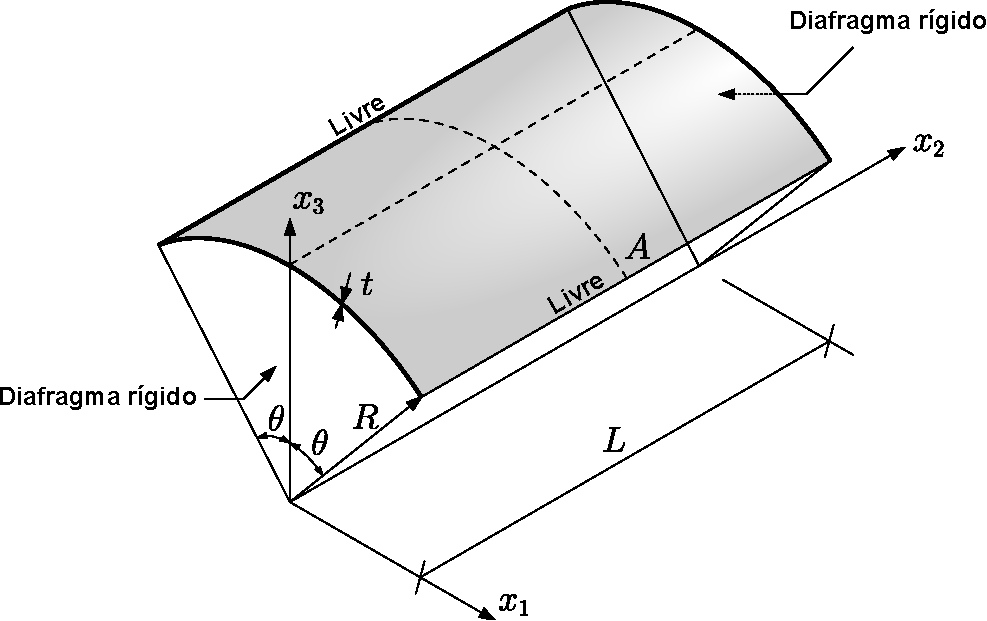
\includegraphics[width=0.75\linewidth]{Figuras/scordelis/scordelis_lo.pdf}
    \\Fonte: Autoria Própria (\the\year).
    \label{fig:scordelis}
\end{figure}

Para a simulação do problema aproveitou-se da simetria da cobertura, o que possibilitou a modelagem de apenas um quarto do problema. Assim utilizou-se uma malha estruturada com orientação à esquerda contendo 512 elementos triangulares de aproximação quadrática, resultando em 7623 graus de liberdade. A malha é apresentada na Figura \ref{fig:scordelis-mesh}. O problema foi considerado em pequenos deslocamentos e deformações, ou seja, utilizou-se somente uma iteração de Newton-Raphson.

\begin{figure}[h!]
    \centering
    \caption{\textit{Scordelis-Lo roof} - Malha utilizada.}
    \begin{subfigure}{0.35\textwidth}
        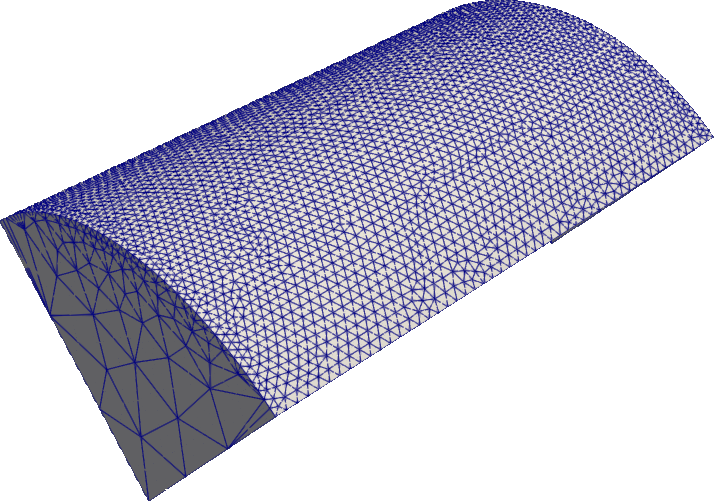
\includegraphics[width=\linewidth]{Figuras/scordelis/malha1.png}
        \caption{Perspectiva isométrica.}
    \end{subfigure}
    \begin{subfigure}{0.35\textwidth}
        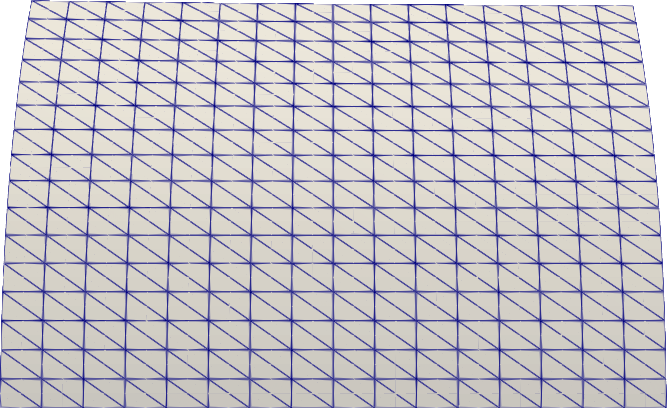
\includegraphics[width=\linewidth]{Figuras/scordelis/malha2.png}
        \caption{Vista superior.}
    \end{subfigure}
    \\Fonte: Autoria Própria (\the\year).
    \label{fig:scordelis-mesh}
\end{figure}

Dessa forma, chegou-se a um deslocamento de 0,2997 nos cálculos realizados, representando um desvio de 0,8965\% em relação à referência. A Figura \ref{fig:scordelis-displ} apresenta o campo de deslocamentos obtido para um quadrante da cobertura.

\begin{figure}[h!]
    \centering
    \caption{\textit{Scordelis-Lo roof} - Campos de deslocamentos obtidos.}
    \begin{subfigure}{0.05\textwidth}
        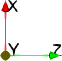
\includegraphics[width=\linewidth]{Figuras/scordelis/eixos.png}
    \end{subfigure}
    \begin{subfigure}{0.31\textwidth}
        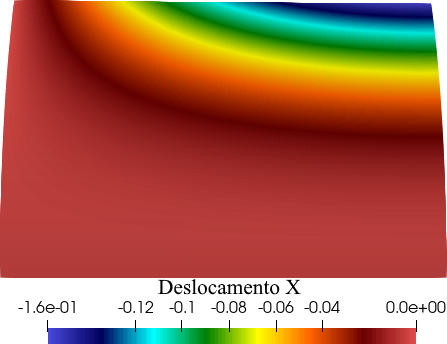
\includegraphics[width=\linewidth]{Figuras/scordelis/ux.png}
    \end{subfigure}
    \begin{subfigure}{0.31\textwidth}
        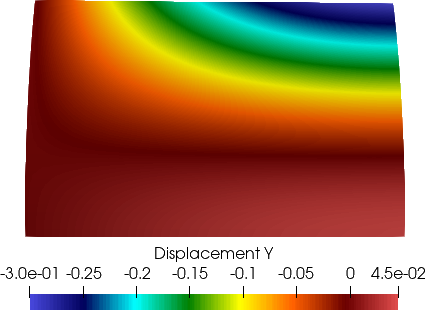
\includegraphics[width=\linewidth]{Figuras/scordelis/uy.png}
    \end{subfigure}
    \begin{subfigure}{0.31\textwidth}
        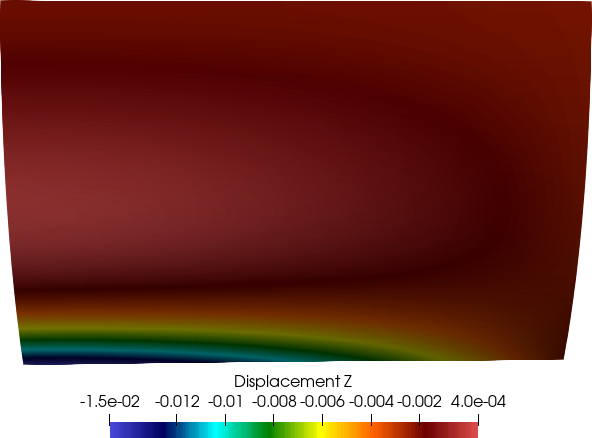
\includegraphics[width=\linewidth]{Figuras/scordelis/uz.png}
    \end{subfigure}
    \\Fonte: Autoria Própria (\the\year).
    \label{fig:scordelis-displ}
\end{figure}

Assim, observa-se que tais campos estão muito semelhantes aos apresentados por \citeonline{ZHOU2022108568}, sendo satisfatoriamente verificada a análise realizada.

Também realizou-se uma análise quanto à dependência da malha, onde dividiu-se as arestas do problema em $N$ partes. A Tabela \ref{tab:scordelis-sol} apresenta os resultados obtidos, sendo os valores do desvio relativo em função do tamanho do elemento ($h$) ilustrados na Figura \ref{fig:shell-static-sol}.

\begin{table}[h!]
    \centering
    \caption{\textit{Scordelis-Lo roof} - Análise da dependência da malha.}
    \begin{tabular}{cccccc}
        \hline
        $N$ & $h$   & Número de elementos & Graus de liberdade & Calculado & Desvio relativo \\\hline
        5   & 5,296 & 50                  & 847                & 0,2258    & 25,3287\%       \\
        6   & 4,413 & 72                  & 1183               & 0,2563    & 15,2354\%       \\
        7   & 3,783 & 98                  & 1575               & 0,2736    & 9,5248\%        \\
        8   & 3,310 & 128                 & 2023               & 0,2835    & 6,2563\%        \\
        9   & 2,942 & 162                 & 2527               & 0,2893    & 4,3178\%        \\
        10  & 2,648 & 200                 & 3087               & 0,2930    & 3,1194\%        \\
        11  & 2,407 & 242                 & 3703               & 0,2953    & 2,3479\%        \\
        12  & 2,207 & 288                 & 4375               & 0,2968    & 1,8323\%        \\
        13  & 2,037 & 338                 & 5103               & 0,2979    & 1,4759\%        \\
        14  & 1,891 & 392                 & 5887               & 0,2987    & 1,2219\%        \\
        15  & 1,765 & 450                 & 6727               & 0,2993    & 1,0360\%        \\
        16  & 1,655 & 512                 & 7623               & 0,2997    & 0,8965\%        \\\hline
    \end{tabular}
    \\Fonte:Autoria Própria (\the\year).
    \label{tab:scordelis-sol}
\end{table}

\begin{figure}[h!]
    \centering
    \caption{\textit{Scordelis-Lo roof} - Desvio relativo do deslocamento vertical do ponto $A$ em função do tamanho do elemento.}
    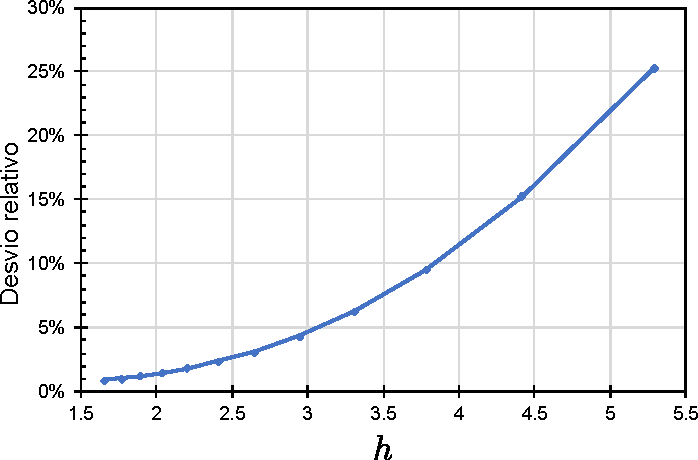
\includegraphics[width=0.6\linewidth]{Figuras/scordelis/static-sol.pdf}
    \\Fonte: Autoria Própria (\the\year).
    \label{fig:shell-static-sol}
\end{figure}

Igualmente realizou-se  uma análise por meio do \textit{software} ANSYS, onde se modelou o problema utilizando uma malha com 648 elementos de casca (\textit{Shell} 281) e 1357 nós, resultando em 8142 graus de liberdade. A Figura \ref{fig:scordelisANSYS} apresenta a malha utilizada na simulação. Assim obteve-se um deslocamento vertical de 0,3016, o que representa um desvio relativo de 0,6300\% em relação ao calculado pelo código implementado. Além disso, observou-se os deslocamentos verticais ao longo da aresta livre da cobertura, os quais são apresentados na Figura \ref{fig:scordelis-graph}.

\begin{figure}[h!]
    \centering
    \caption{\textit{Scordelis-Lo roof} - Malha utilizada no ANSYS.}
    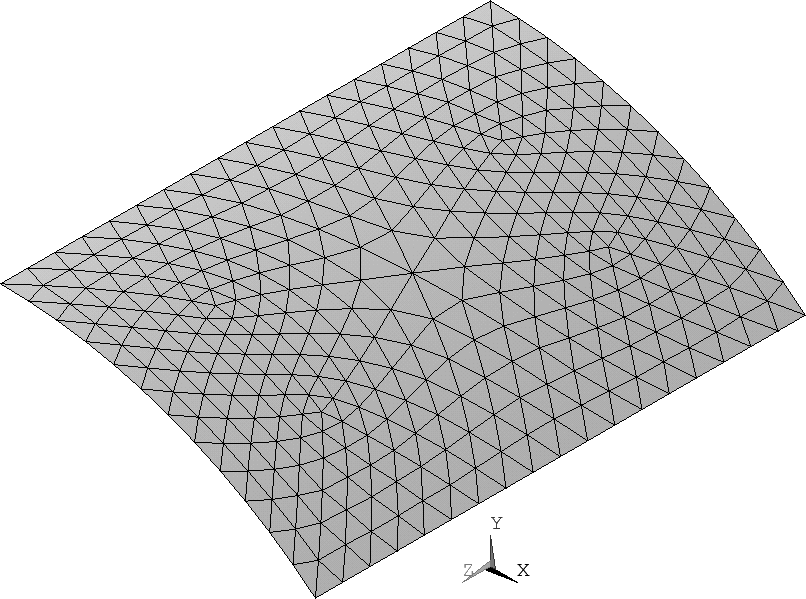
\includegraphics[width=0.45\linewidth]{Figuras/scordelis/ANSYS.png}
    \\Fonte: ANSYS (\the\year).
    \label{fig:scordelisANSYS}
\end{figure}

\begin{figure}[h!]
    \centering
    \caption{\textit{Scordelis-Lo roof} - Deslocamento vertical ao longo da aresta livre.}
    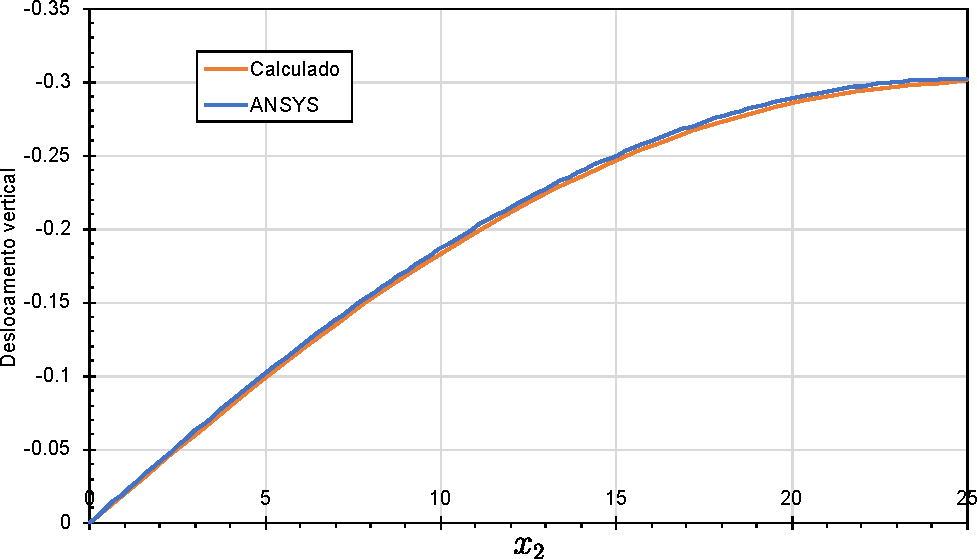
\includegraphics[width=0.6\linewidth]{Figuras/scordelis/deslocamento.pdf}
    \\Fonte: Autoria Própria (\the\year).
    \label{fig:scordelis-graph}
\end{figure}

% =============================================================================
\subsection{Cilindro biengastado em problema estático} \label{Ap:Shell-cyl}
% =============================================================================

Outro problema comum considera um cilindro sujeito a duas cargas concentradas diametralmente opostas, conforme visto na Figura \ref{fig:cylinder-shell}. As dimensões do problema são: comprimento $L=600$, raio $R=300$ e espessura $t=3$. A carga aplicada é $P=1$. O material que constitui o cilindro possui módulo de elasticidade $E=3\times10^6$ e coeficiente de Poisson $\nu=0,3$. Ambas as extremidades do cilindro estão vinculadas a um diafragma rígido, ou seja, $u_1=u_3=\phi_2=0$. O resultado de referência adotado é de um deslocamento radial de $1,8248\times10^{-5}$ no ponto de aplicação da carga \cite{BELYTSCHKO1985221,CHAUDINH2023110222,ZHOU2022108568}.

\begin{figure}[h!]
    \centering
    \caption{Cilindro biengastado em problema estático - Desenho esquemático.}
    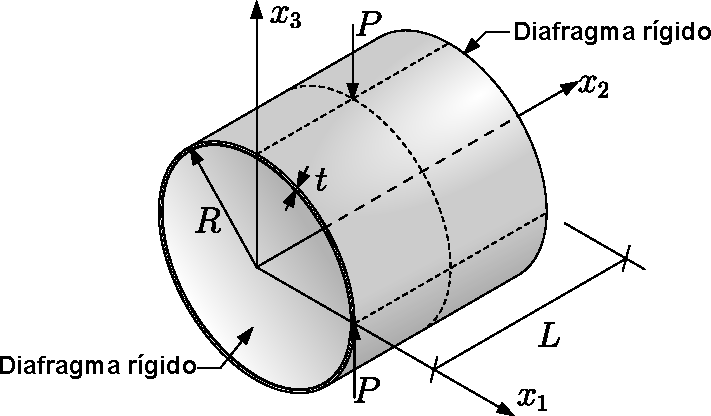
\includegraphics[width=0.65\linewidth]{Figuras/cylinder-shell/cylinder.pdf}
    \\Fonte: Autoria Própria (\the\year).
    \label{fig:cylinder-shell}
\end{figure}

Pelo fato de o problema apresentar simetria, foi estudado somente um octante do problema. Assim utilizou-se uma malha não-estruturada, com refinamento maior próximo ao ponto de aplicação da força, contendo 810 elementos triangulares de aproximação quadrática, contando com um total de 11977 graus de liberdade. A malha utilizada é observada na Figura \ref{fig:cylinder-shell-mesh}. Na simulação adotou-se uma única iteração de Newton-Raphson.

\begin{figure}[h!]
    \centering
    \caption{Cilindro biengastado em problema estático - Malha utilizada.}
    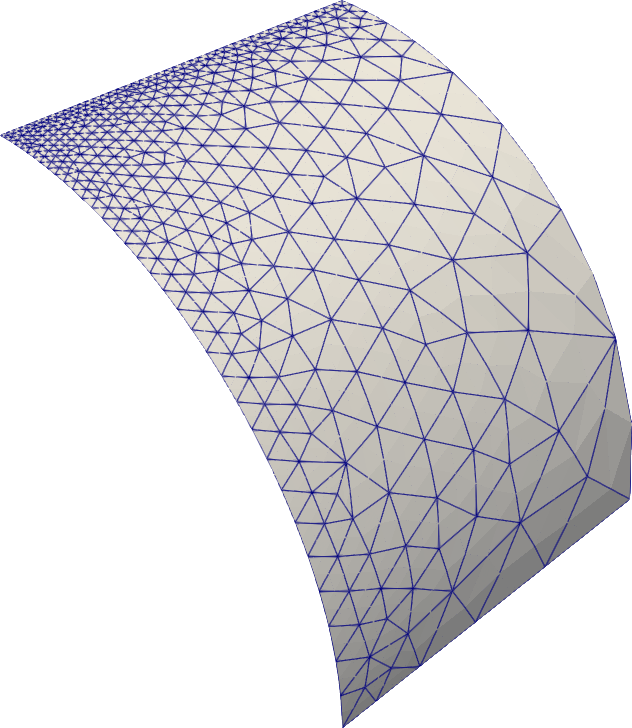
\includegraphics[width=0.3\linewidth]{Figuras/cylinder-shell/mesh1.png}
    \\Fonte: Autoria Própria (\the\year).
    \label{fig:cylinder-shell-mesh}
\end{figure}

O resultado obtido foi de um deslocamento radial de $1,8135\times10^{-5}$, tendo, portanto, um desvio relativo de $0,6176\%$ em relação à referência. Os campos de deslocamentos obtidos são apresentados na Figura \ref{fig:cylinder-shell-disp}, os quais são muito próximos aos obtidos por \citeonline{ZHOU2022108568}.

\begin{figure}[h!]
    \centering
    \caption{Cilindro biengastado em problema estático - Campos de deslocamentos obtidos.}
    \begin{subfigure}{0.075\textwidth}
        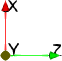
\includegraphics[width=\linewidth]{Figuras/cylinder-shell/eixos.png}
    \end{subfigure}
    \begin{subfigure}{0.3\textwidth}
        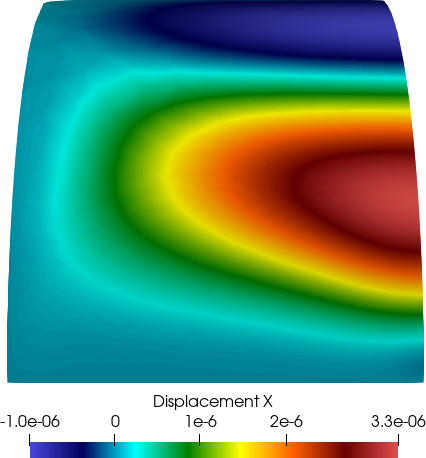
\includegraphics[width=\linewidth]{Figuras/cylinder-shell/ux.png}
    \end{subfigure}
    \begin{subfigure}{0.3\textwidth}
        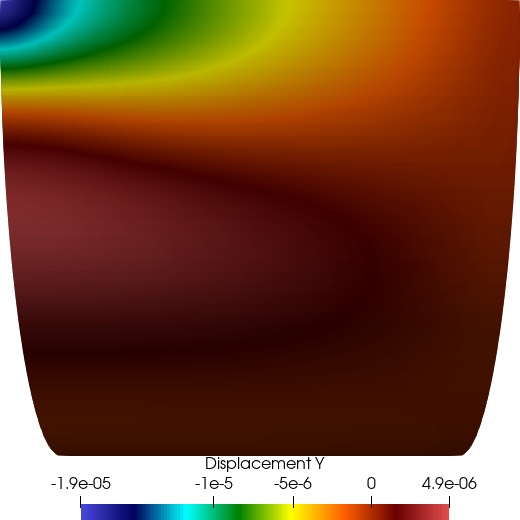
\includegraphics[width=\linewidth]{Figuras/cylinder-shell/uy.png}
    \end{subfigure}
    \begin{subfigure}{0.3\textwidth}
        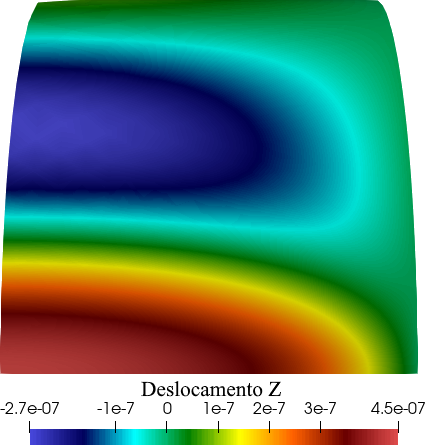
\includegraphics[width=\linewidth]{Figuras/cylinder-shell/uz.png}
    \end{subfigure}
    \\Fonte: Autoria Própria (\the\year).
    \label{fig:cylinder-shell-disp}
\end{figure}

Também se comparou o resultado obtido com relação à uma simulação feita no \textit{software} ANSYS, onde modelou-se uma malha contendo 2592 elementos \textit{Shell} 281, com um total de 5305 nós e 31830 graus de liberdade. A Figura \ref{fig:clampedCylinderANSYS} apresenta a malha utilizada. Assim obteve-se um deslocamento de $1,8142\times10^{-5}$, resultando em um desvio relativo de $0,03858\%$. Além disso, verificou-se o deslocamento radial ao longo das arestas compreendidas pela interseção do cilindro com o plano $x_1=0$ e com $x_2=L/2$. A Figura \ref{fig:cylinder-shell-deslradial} ilustra graficamente os resultados obtidos.

\begin{figure}[h!]
    \centering
    \caption{Cilindro biengastado em problema estático - Malha utilizada no ANSYS.}
    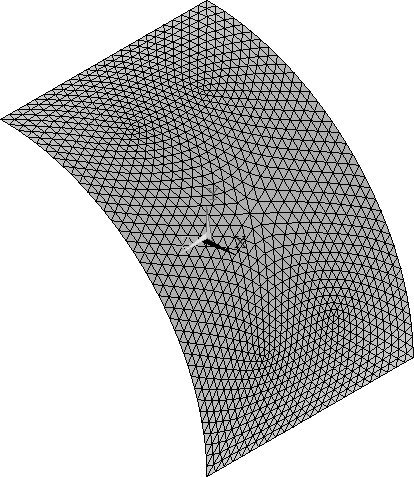
\includegraphics[width=0.35\linewidth]{Figuras/cylinder-shell/ANSYS.png}
    \\Fonte: ANSYS (\the\year).
    \label{fig:clampedCylinderANSYS}
\end{figure}

\begin{figure}[h!]
    \centering
    \caption{Cilindro biengastado em problema estático - Deslocamentos radiais.}
    \begin{subfigure}{0.49\textwidth}
        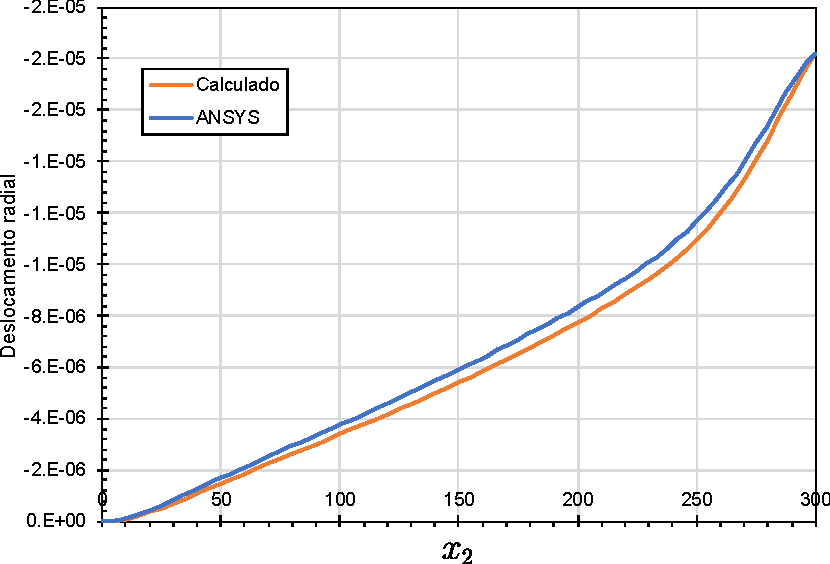
\includegraphics[width=\linewidth]{Figuras/cylinder-shell/deslocamento1.pdf}
        \caption{Interseção com o plano $x_1=0$}
    \end{subfigure}
    \begin{subfigure}{0.49\textwidth}
        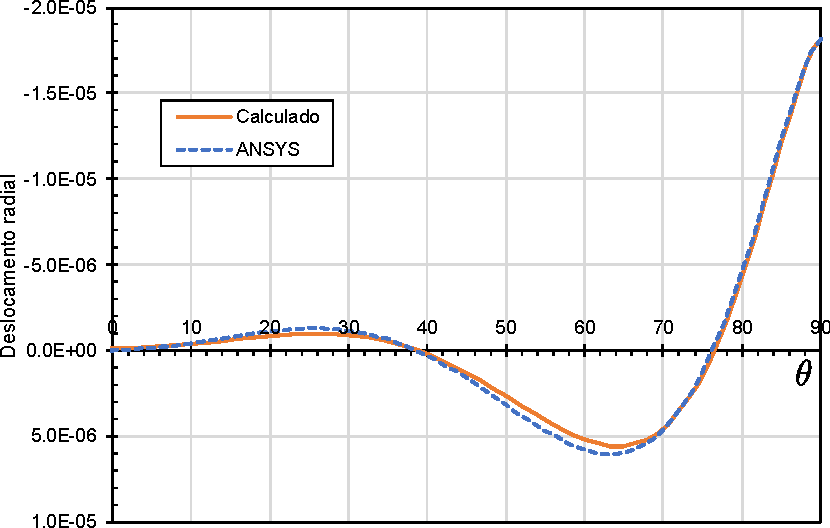
\includegraphics[width=\linewidth]{Figuras/cylinder-shell/deslocamento2.pdf}
        \caption{Interseção com o plano $x_2=L/2$}
    \end{subfigure}
    \\Fonte: Autoria Própria (\the\year).
    \label{fig:cylinder-shell-deslradial}
\end{figure}

% =============================================================================
\subsection{Viga engastada em problema dinâmico} \label{Ap:DinBeam}
% =============================================================================

Para verificação do código implementado em problemas dinâmicos, estudou-se  primeiramente o comportamento de uma viga engastada em uma de suas extremidades e sujeita a uma carga $P$ aplicada na extremidade oposta, conforme ilustrado na Figura \ref{fig:viga1}. As dimensões da viga são: comprimento $L=60$ dm, altura $h=3$ dm e largura $b=1$ dm. A força aplicada possui intensidade $P=1,25\times10^{-4}$ Mg$\cdot$dm/(ms)² $\script{H}(t)$, sendo $\script{H}(t)$ a função de Heaviside. O material que compõe a viga possui módulo de Young $E=20$ Mg/[dm$\cdot$(ms)²], coeficiente de Poisson nulo e massa específica $\rho=7\times10^{-3}$ Mg/dm³. O intervalo de tempo analisado foi $t\in[0;675]$ ms discretizado em passos de tempo $\Delta t=0,3377$ ms, sendo utilizado um raio espectral $\rho_\infty=1,0$. A malha de elementos finitos utilizada conta com 32 elementos triangulares de aproximação quadrática, com um total de 99 nós e 693 graus de liberdade, a qual pode ser observada na Figura \ref{fig:viga1-mesh}.

\begin{figure}[h!]
    \centering
    \caption{Viga engastada em problema dinâmico - Desenho esquemático.}
    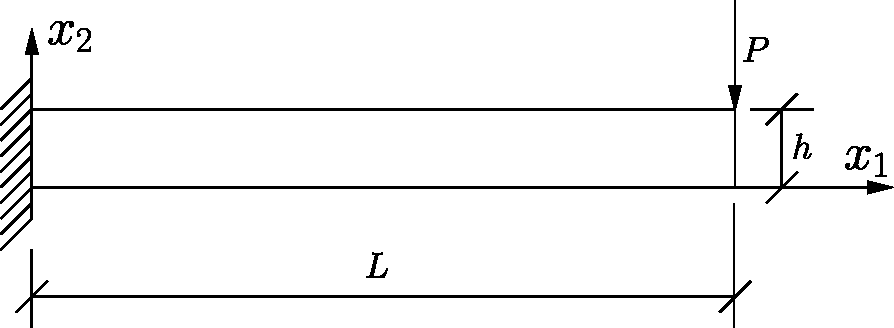
\includegraphics[width=0.5\linewidth]{Figuras/vigas/viga1.pdf}
    \\Fonte: Autoria Própria (\the\year).
    \label{fig:viga1}
\end{figure}

\begin{figure}[h!]
    \centering
    \caption{Viga engastada em problema dinâmico - Malha utilizada.}
    
\includegraphics[width=\linewidth]{Figuras/vigas/mesh1.png}
    \\Fonte: Autoria Própria (\the\year).
    \label{fig:viga1-mesh}
\end{figure}

A modelagem realizada considerou a altura $H$ como a espessura do elemento de casca, sendo a força atuante nessa mesma direção. Assim, observou-se o deslocamento vertical no ponto de aplicação da força. Os resultados obtidos foram comparados com aqueles alcançados a partir de uma modelagem no \textit{software} ANSYS utilizando 346 elementos do tipo \textit{Shell} 281, totalizando 795 nós e 4770 graus de liberdade (Figura \ref{fig:beamANSYS1}). a Figura \ref{fig:res-viga1} apresenta os resultados calculados.

\begin{figure}[h!]
    \centering
    \caption{Viga engastada em problema dinâmico - Malha utilizada no ANSYS.}
    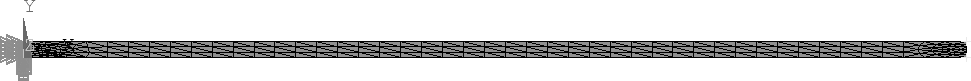
\includegraphics[width=\linewidth]{Figuras/vigas/ANSYSmesh1.png}
    \\Fonte: ANSYS (\the\year).
    \label{fig:beamANSYS1}
\end{figure}

\begin{figure}[h!]
    \centering
    \caption{Viga engastada em problema dinâmico - Deslocamento vertical no ponto de aplicação da força ao longo do tempo.}
    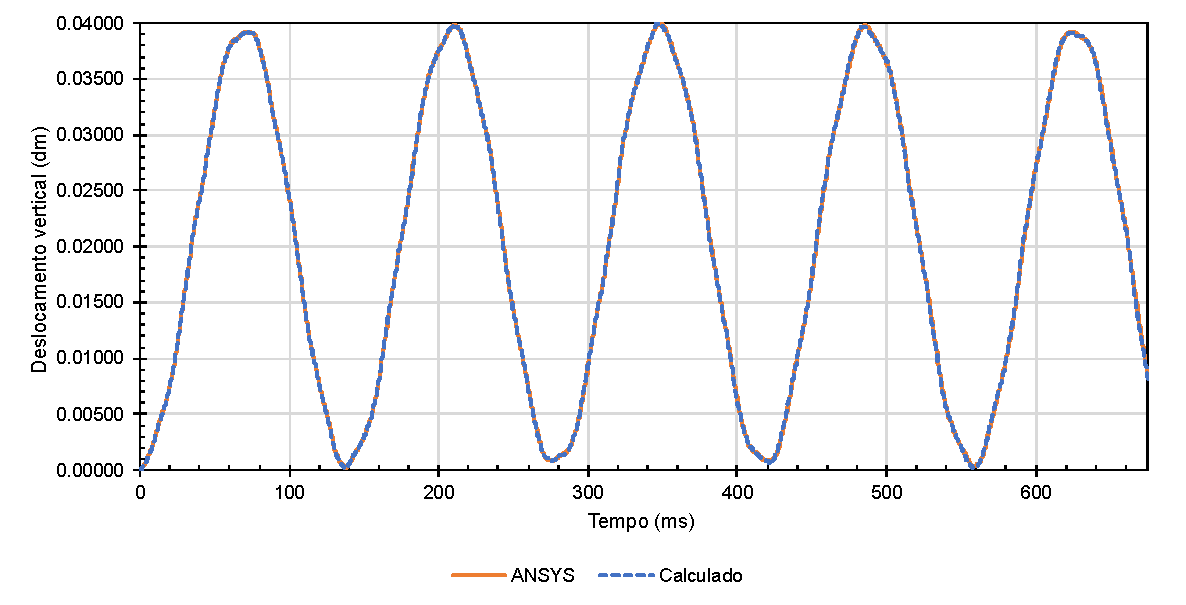
\includegraphics[width=.8\linewidth]{Figuras/vigas/res1.pdf}
    \\Fonte: Autoria Própria (\the\year).
    \label{fig:res-viga1}
\end{figure}

Observa-se nesse caso uma boa concordância entre os resultados apresentados pelo ANSYS e os obtidos pelo código desenvolvido, sendo verificada a eficácia nesse exemplo.

% =============================================================================
\subsection{Viga biengastada em problema dinâmico} \label{Ap:DinBeam2}
% =============================================================================

Outro exemplo trata-se de uma viga biengastada com uma carga aplicada em seu centro, conforme mostrado na Figura \ref{fig:viga2}. Nesse exemplo considerou-se um comprimento $L=20$ in, com seção transversal de $b\times h=1,0\times0,125$ in². O material que constitui a viga possui módulo de Young $E=3\times10^{7}$ lb/in², coeficiente de Poisson nulo e massa específica de $\rho=2,6\times10^{-4}$ lb$\cdot$s²/in$^4$. A força aplicada foi de $P=640$ lb constante durante todo o período de análise, de $t\in[0;5]$ ms, o qual foi discretizado em passos de tempo de $\Delta t=25\ \mu$s. O esquema de integração temporal deu-se ao considerar $\rho_\infty=1,0$. A malha de elementos finitos (Figura \ref{fig:viga2-mesh}) possui 132 elementos triangulares de aproximação quadrática, totalizando 333 nós e 2331 graus de liberdade. A espessura do elemento de casca foi considerada como a direção da altura $H$ da viga.

\begin{figure}[h!]
    \centering
    \caption{Viga biengastada em problema dinâmico - Desenho esquemático.}
    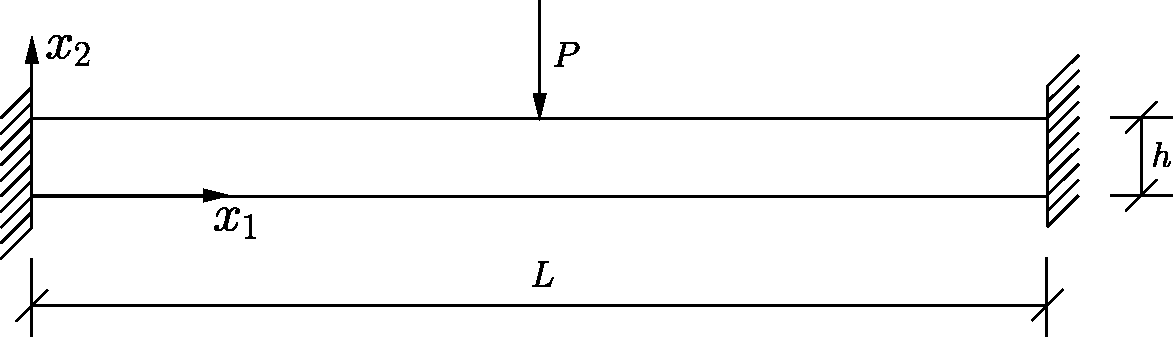
\includegraphics[width=0.6\linewidth]{Figuras/vigas/viga2.pdf}
    \\Fonte: Autoria Própria (\the\year).
    \label{fig:viga2}
\end{figure}

\begin{figure}[h!]
    \centering
    \caption{Malha utilizada na simulação da viga biengastada.}
    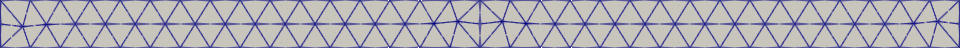
\includegraphics[width=\linewidth]{Figuras/vigas/mesh2.png}
    \\Fonte: Autoria Própria (\the\year).
    \label{fig:viga2-mesh}
\end{figure}

Os resultados calculados foram comparados com os apresentados pelo ANSYS, a partir de 234 elementos do tipo \textit{Shell} 281, resultando em 541 nós e 3246 graus de liberdade (Figura \ref{fig:beamANSYS2}), e por \cite{mondkar1977ansa}. A Figura \ref{fig:res-viga2} exibe os resultados obtidos.

\begin{figure}[h!]
    \centering
    \caption{Viga biengastada em problema dinâmico - Malha utilizada no ANSYS.}
    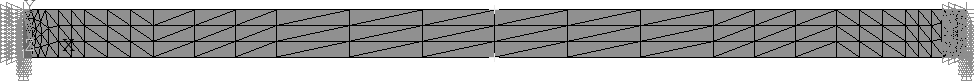
\includegraphics[width=\linewidth]{Figuras/vigas/ANSYSmesh2.png}
    \\Fonte: ANSYS (\the\year).
    \label{fig:beamANSYS2}
\end{figure}

\begin{figure}[h!]
    \centering
    \caption{Viga biengastada em problema dinâmico - Deslocamento vertical no centro da viga biengastada ao longo do tempo.}
    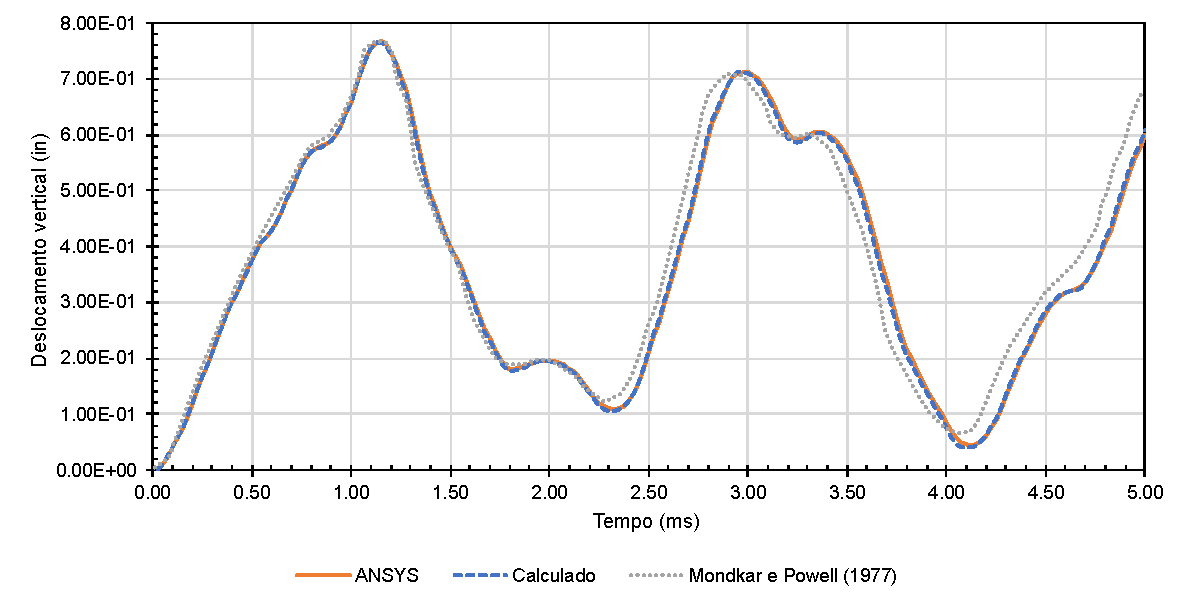
\includegraphics[width=\linewidth]{Figuras/vigas/res2.pdf}
    \\Fonte: Autoria Própria (\the\year).
    \label{fig:res-viga2}
\end{figure}

Verifica-se uma boa concordância entre os resultados obtidos pela análise por ambos os valores de referência, sendo assim, averiguada a eficácia do código nesse exemplo.